\documentclass[12pt]{article} %Styl dokumentu
\usepackage{times} %Czcionka
\usepackage[a4paper,left=3.5cm,right=2.5cm,top=3cm,bottom=3cm,includefoot=false,includehead=false]{geometry} %Ustawienia marginesów
\linespread{1} %Interlinia
\setlength{\parindent}{0.5cm} %Wcięcie na początku akapitu
\setlength{\parskip}{1ex plus 0.5ex minus 0.2ex} %Odstępy pomiędzy akapitami

%Dodatkowe pakiety ******************************************************************
\usepackage[T1]{fontenc} %Styl tytułów rozdziałów
%\usepackage{subfig} NIE WIEM DO CZEGO ALE W PRZEJŚCIÓWCE TO MIAŁEM
%\usepackage{float} COS Z FLOATAMI ALE NIE WIEM CO, MOŻE NIE BĘDZIE NAM POTRZEBNE
\usepackage{amsfonts} %Niektóre symbole matematyczne
\usepackage{fixltx2e} %subscript
%\usepackage{pdfpages} %Dołączanie pdfów do tekstu
\usepackage{listings} %Pakiet od listingów programów
\usepackage{xcolor} %Pakiet kolorów do listingów programów Arduino
\usepackage{amsmath} %Pakiet matematyczny
\usepackage{bm,array} %Pakiet do tabel
\usepackage{fancyhdr} %Nagłówek i stopka
\usepackage{graphicx} %Wykresy i obrazy
\usepackage{subfigure} %Dodatkowa biblioteka do obrazów
\usepackage{polski} %Ustawienie języka polskiego
\usepackage[utf8]{inputenc} %Ustawienie kodowania polskich znaków
\usepackage{hyperref} %hiperłącza
\usepackage[labelfont=it,textfont={it}]{caption} %Formatowanie podpisów tabel i rysunków
\usepackage{wrapfig} %tekst obok rysunków
\usepackage{multirow}

%Definiowanie stylu Arduino dla listings*********************************************
\usepackage{xcolor}
\definecolor{dkgreen}{rgb}{0,0.6,0}
\definecolor{dred}{rgb}{0.545,0,0}
\definecolor{dblue}{rgb}{0,0,0.545}
\definecolor{lgrey}{rgb}{0.95,0.95,0.95}
\definecolor{gray}{rgb}{0.4,0.4,0.4}
\definecolor{darkblue}{rgb}{0.0,0.0,0.6}
\definecolor{ArdOr}{rgb}{1,0.451,0.0}
\lstdefinelanguage{Arduino}{
      backgroundcolor=\color{lgrey},  
      basicstyle=\footnotesize \ttfamily \color{black} \bfseries,   
      breakatwhitespace=false,       
      breaklines=true,               
      captionpos=b,                   
      commentstyle=\color{dkgreen},   
      deletekeywords={...},          
      escapeinside={\%*}{*)},                  
      frame=single,                  
      language=C++,                
      keywordstyle=\color{ArdOr},  
      morekeywords={BRIEFDescriptorConfig,string,TiXmlNode,DetectorDescriptorConfigContainer,istringstream,cerr,exit}, 
      identifierstyle=\color{black},
      stringstyle=\color{blue},      
      numbers=left,                 
      numbersep=5pt,                  
      numberstyle=\color{black}, 
      rulecolor=\color{black},        
      showspaces=false,               
      showstringspaces=false,        
      showtabs=false,                
      stepnumber=1,                   
      tabsize=5,                     
      title=\lstname,                 
    }

%Nadpisywanie komend****************************************************************
\renewcommand{\theequation}{\thesubsection.\arabic{equation}}
\numberwithin{equation}{subsection}
\renewcommand{\thefigure}{\thesection.\arabic{figure}}
\renewcommand{\figurename}{Rys.} 
\numberwithin{figure}{section}
\renewcommand{\thetable}{\thesection.\arabic{table}}
\numberwithin{table}{section}
\renewcommand{\captionfont}{\small}
\renewcommand{\lstlisting}{\thesubsection.\arabic{lstlisting}}
\let\stdsection\subsection


\begin{document}

%---------------------------------------------------STRONA TYTUŁOWA-------------------------------------------------------------

\begin{center}
	\large{INSTYTUT AUTOMATYKI\\I INŻYNIERII INFORMATYCZNEJ\\WYDZIAŁ ELEKTRYCZNY\\POLITECHNIKA POZNAŃSKA\\}
\end{center}
\vspace{2cm} 
\begin{center}
	INŻYNIERSKA PRACA DYPLOMOWA\\
\end{center}
\begin{center}
	\Large{\textbf{SYSTEM WSPOMAGAJĄCY KIEROWANIE POJAZDEM\\Z UŻYCIEM ZŁĄCZA DIAGNOSTYCZNEGO}}
\end{center}
\begin{center}
	\large{\textbf{Mateusz BARTOSZ}}
\end{center}
\vspace{4cm}
\begin{flushright}
	Promotor:\\\textbf{Dr inż. Konrad URBAŃSKI}\\
\end{flushright}
\vspace{4cm} 
\begin{center}
	Poznań 2017
\end{center}

%---------------------------------------------------POCZĄTEK DOKUMENTU-------------------------------------------------------------

\thispagestyle{empty}
\newpage
%
%\pagestyle{fancy}
%\rhead{\thepage}
%\lhead{\slshape \rightmark}
%\lfoot{}
%\cfoot{}
%\rfoot{}
%
%\begin{flushright}
%\vspace{4cm}
%\textit{\large{
%\\ 
%\vspace{17cm}
%Składam serdeczne podziękowania\\
%Panu dr. inż. Konradowi Urbańskiemu\\ 
%za cierpliwość, poświęcony czas\\ 
%oraz bezcenne uwagi merytoryczne.}}
%\end{flushright}
%\newpage
\tableofcontents
\thispagestyle{empty}

%---------------------------------------------------STRESZCZENIE-------------------------------------------------------------
\newpage
\thispagestyle{empty}
\section*{Streszczenie}
\vspace{0.5cm}
\hspace{0.5cm}
\newpage

\section*{Abstract}
\thispagestyle{empty}
\vspace{0.5cm}
\hspace{0.5cm}

\newpage

%---------------------------------------------------WSTĘP-------------------------------------------------------------
\section{Wstęp}

	\subsection{Wybór tematu}
		\hspace{0.5cm}Głównym czynnikiem decydującym o wyborze tematu było zainteresowanie rozwiązaniami elektronicznymi stosowanymi we współczesnej motoryzacji oraz chęć podjęcia próby zbudowania układu opartego o własną koncepcję pracującego jako komputer pokładowy w samochodzie osobowym. Kolejnym czynnikiem było umożliwienie ciągłego badania i kontroli parametrów pracy poszczególnych układów pojazdu, w celu uniknięcia, lub wczesnego wykrycia potencjalnych usterek. Dodatkową motywacją była chęć zbudowania układu, który mógłby być w przyszłości praktycznie wykorzystywany w samochodach niewyposażonych w wbudowany komputer pokładowy. 	
	
	\subsection{Cel i zakres pracy}
		\hspace{0.5cm}Celem pracy było zaprojektowanie oraz wykonanie układu przyłącza do gniazda diagnostycznego w samochodzie osobowym Seat Cordoba III oraz zbudowanie interfejsu użytkownika umożliwiającego wizualizację odczytywanych parametrów, kontrolę wartości granicznych, a także przechowanie ich w celach dalszej diagnostyki. Dodatkowym celem było określenie możliwości wykorzystania odbieranych parametrów do opracowania algorytmów umożliwiających wspomaganie kierującego pojazdem, aby zoptymalizować jazdę, zwiększyć bezpieczeństwo podróży oraz zminimalizować ryzyko wystąpienia usterek. 
	
	\subsection{Założenia i wymagania}
		\hspace{0.5cm}Założeniem pracy jest opracowanie kompleksowego układu umożliwiającego odczytywanie, wizualizację oraz kontrolę parametrów odbieranych przez złącze diagnostyczne w samochodzie osobowym Seat Cordoba III, a także określenie możliwości wykorzystania tych parametrów do opracowania algorytmów wspomagających prowadzenie pojazdu.
	
		\newpage

%---------------------------------------------------ZAGADNIENIA WPROWADZAJĄCE-------------------------------------------------------------
\section{Zagadnienia wprowadzające}
	\hspace{0.5cm}We współczesnej motoryzacji wyraźnie można zauważyć tendencję automatyzacji procesu prowadzenia pojazdu oraz kontroli stanu jego parametrów. W samochodach dostępnych na rynku można spotkać bardzo wiele różnych protokołów komunikacyjnych. Cześć z nich służy do komunikacji pomiędzy urządzeniami wewnętrznymi pojazdu, inne do komunikacji z użytkownikiem, w celu zwiększenia komfortu jazdy, a jeszcze inne wykorzystywane są w diagnostyce stanu poszczególnych układów samochodu. Te ostatnie, wyprowadzone są do gniazda diagnostycznego(ang. On-Board Diagnosdic - OBD). W zależności od producenta, modelu oraz roku produkcji pojazdu do dyspozycji są różne protokoły. Umożliwiają one między innymi odczytywanie aktualnych wskazań niektórych czujników, kontrolę zużywania się elementów eksploatacyjnych czy detekcję błędów silnika. W niniejszym rozdziale omówione zostało złącze diagnostyczne w wersji drugiej(ODB2) wraz z udostępnianymi przez nie protokołami komunikacyjnymi. Dodatkowo w ostatnim podrozdziale znajduje się przegląd narzędzi wykorzystanych podczas realizacji pracy.

	\subsection{Złącze diagnostyczne}
		\hspace{0.5cm}Historia złącza diagnostycznego używanego w motoryzacji sięga końcówki lat sześćdziesiątych dwudziestego wieku. Pierwsze komputery pokładowe wprowadzone zostały w samochodach marki Volkswagen w 1968 roku. Dziesięć lat później za sprawą marki Nissan komputery pokładowe pojawiły się w pojazdach konsumenckich. Kolejnym krokiem było wprowadzenie protokołu ALDL  przez General Motors w 1980 roku. Był to pierwszy standard zbliżony do obecnie stosowanego w gniazdach OBD2. Występował w trzech wersjach: dwunasto, dziesięcio i pięciopinowej. Pierwsze wersje były jednokierunkowe i umożliwiały przesyłanie 160 bodów danych. W późniejszych wersjach wprowadzono dwukierunkową transmisję danych o zwiększono szybkości transmisji do 8192 bodów. W 1991 roku agencja California Air Resources Board zażądała, aby każdy nowy pojazd sprzedawany w Kalifornii posiadał wyprowadzenie diagnostyczne. Stało się to impulsem do opracowania i wprowadzenia standardu OBD-I, choć nazwa ta została wprowadzona dopiero po opracowaniu kolejnego standardu OBD w wersji drugiej. Złącze ODB-I nie zostało ściśle ustandaryzowane i każdy producent samochodów mógł wykonać je w swojej wersji. Główną motywacją do wprowadzenia tego standardu było zachęcenie producentów pojazdów do zaprojektowania systemów kontroli emisji spalin. Często spotykana wersja tego złącza umożliwiała odczytywanie kodów błędów poprzez analizę migania diody znajdującej się przy złączu. Miganie diody reprezentowało odpowiednią liczbę dwucyfrową, która była interpretowana jako odpowiedni kod błędu pojazdu. W 1994 roku na bazie poprawionej i uzupełnionej specyfikacji OBD-I powstał standard OBD w wersji drugiej - ODB-II. Jest to najpopularniejszy, aktualnie używany system diagnostyki samochodowej. Od roku 1996 wszystkie nowe samochody sprzedawane w Stanach Zjednoczonych muszą być wyposażone właśnie w gniazdo ODB w wersji drugiej. W 2001 roku standard OBD-II pod nazwą EOBD został wprowadzony jako obowiązkowy w samochodach benzynowych produkowanych w Unii Europejskiej, a w 2003 roku również w samochodach z silnikami wysokoprężnymi.
		
		\newpage
		
		\subsubsection{Złącze diagnostyczne OBD-II}
			\hspace{0.5cm}Złącze diagnostyczne OBD w wersji drugiej jest aktualnie stosowanym w motoryzacji wyprowadzeniem umożliwiającym wykrywanie błędów poszczególnych układów pojazdu. Opis budowy tego złącza zawarty jest w normie SAE J1962[\cite{saej1962}]. Standard OBD-II zawiera specyfikację dotyczącą budowy złącza, a także opis udostępnianych przez nie protokołów komunikacyjnych. Zgodnie z normą, złącze występuje w dwóch wersjach: A oraz B, oba szesnastopinowe (2x8), żeńskie. Na Rys. \ref{rys_obd2_wtyczka} przedstawiono budowę obu typów złączy.
		
		\begin{figure}[ht]
		\centering
		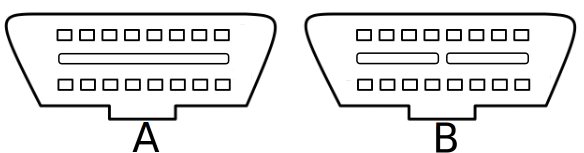
\includegraphics[scale=0.8]{Images/ZlaczaOBD2.pdf}
		\caption{Porównanie złącza diagnostycznego w wersji A oraz B.}
		\label{rys_obd2_wtyczka}
		\end{figure}
		
		Złącze typu A stosowane jest w pojazdach wyposażonych w akumulator o napięciu 12V, natomiast złącze typu B w pojazdach wyposażonych w akumulator o napięciu 24V.
		
		Norma SAE J1962 definiuje protokoły komunikacyjne udostępniane przez złącze diagnostyczne. Dostępność poszczególnych protokołów komunikacyjnych może być różna w zależności od producenta pojazdu oraz roku produkcji. Na Rys. \ref{rys_obd2_pinout} oraz w tabeli \ref{tab_obd2_pinout} przedstawione zostały potencjalnie dostępne protokoły komunikacyjne wraz z numerem pinu, do którego powinny być podłączone.
		
		\begin{figure}[ht]
		\centering
		\includegraphics[scale=0.8]{Images/ZlaczeOBD2_pinout.pdf}
		\caption{Opis wyprowadzeń złącza diagnostycznego. Wykorzystywane wyprowadzenia zostały zaznaczone kolorem niebieskim oraz odpowiednim numerem. Opis wyprowadzeń znajduje się w Tab \ref{tab_obd2_pinout}}
		\label{rys_obd2_pinout}
		\end{figure}
		
		W złączu diagnostycznym udostępnionych jest 5 różnych protokołów. Dodatkowo rozróżnione są dwie masy: masa podwozia oraz masa sygnałowa. W praktyce najczęściej wyprowadzenia te są ze sobą zwarte. Zazwyczaj w pojazdach udostępniony jest tylko jeden z opisanych poniżej protokołów. 
		
		\newpage
		
		\begin{table}[ht]
\centering
\caption{Opis wyprowadzeń złącza diagnostycznego OBD-II.}
\label{tab_obd2_pinout}
\begin{tabular}{|c|c|}
\hline
\textbf{Numer wyprowadzenia} & \textbf{Przeznaczenie wyprowadzenia}                                                                    \\ \hline
2                            & Linia dodatnia protokołu SAE J1850 PWM oraz VPW                                                         \\ \hline
4                            & Masa podwozia                                                                                           \\ \hline
5                            & Masa sygnałowa                                                                                          \\ \hline
6                            & Linia wysoka magistrali CAN                                                                             \\ \hline
7                            & Linia K protokołu ISO 9141-2 oraz ISO 14230-4                                                           \\ \hline
10                           & Linia ujemna protokołu SAE J1850 PWM                                                                    \\ \hline
14                           & Linia niska magistrali CAN                                                                              \\ \hline
15                           & Linia L protokołu ISO 9141-2 oraz ISO 14230-4                                                           \\ \hline
16                           & \begin{tabular}[c]{@{}c@{}}Zasilanie\\ 12V/4A dla złącza typu A\\ 24V/2A dla złącza typu B\end{tabular} \\ \hline
\end{tabular}
\end{table}
		
		\subsubsection{Struktura wysyłanych zapytań}
		
		\hspace{0.5cm}Przy użyciu złącza diagnostycznego można odpytywać komputer pokładowy parametry z dziesięciu podgrup wybierając odpowiedni tryb. Tryby wybierane są za pomocą wysłania w żądaniu odpowiedniej liczby zapisanej w postaci szesnastkowej do złącza diagnostycznego. W tabeli \ref{tab_pid_modes} przedstawionych jest dziesięć modów opisanych w normie SAE J1979.
		
		\begin{table}[ht]
\centering
\caption{Tryby pracy złącza diagnostycznego}
\label{tab_pid_modes}
\begin{tabular}{|c|c|}
\hline
\textbf{Tryb (hex)} & \textbf{Opis}                                                               \\ \hline
01                  & Aktualny stan parametrów poszczególnych układów                             \\ \hline
02                  & Stan niektórych czujników w momencie wystąpienia błędu                      \\ \hline
03                  & Zapisane kody błędów                                                        \\ \hline
04                  & Wyczyszczenie zapisanych kodów błędów            \\ \hline
05                  & Wyniki testu samodiagnostyki czujnika tlenu \\ \hline
06                  & Wyniki testu samodiagnostyki czujnika tlenu (CAN)                             \\ \hline
07                  & Kody błędów z aktualnego oraz poprzedniego przejazdu         \\ \hline
08                  & Kontrola operacji poszczególnych układów wewnętrznych                       \\ \hline
09                  & Parametry pojazdu                                                           \\ \hline
0A                  & Trwałe kody błędów (czyste kody błędów)                                     \\ \hline
\end{tabular}
\end{table}
		
		
		\newpage
		
		\subsubsection{Struktura kodów błędów}
		
	
		\newpage	
	
	\subsection{Protokoły komunikacyjne dostępne w złączu diagnostycznym}
		\hspace{0.5cm}GŁÓWNIE TE Z OBD LIN, ISO9141-2, CAN,
						te nowsze
	
		\newpage	
	
	\subsection{Opis wykorzystanych narzędzi}
		\hspace{0.5cm}
		-java
		-javafx
		-raspberry
		-PCB
	
		\newpage
	
%---------------------------------------------------STRUKTURA PROJEKTU-------------------------------------------------------------	
\section{Struktura projektu}
	\hspace{0.5cm}
	-założenia całościowe
	-schemat
	-opis ogólny	
	
	\newpage	
	
%---------------------------------------------------PROJEKT PŁYTKI-------------------------------------------------------------	
\section{Projekt układu do komunikacji ze złączem diagnostycznym}
	\subsection{Schemat elektryczny}
		\hspace{0.5cm}
	
		\newpage
	
	\subsection{Projekt płytki drukowanej}
		\hspace{0.5cm}
	
		\newpage
%---------------------------------------------------APLIKACJA KOMUNIKACYJNA-------------------------------------------------------------	
	
\section{Aplikacja przetwarzająca dane ze złącza diagnostycznego}
	\hspace{0.5cm}
	
	\newpage
	
%---------------------------------------------------INTERFEJS GRAFICZNY-------------------------------------------------------------	
	
\section{Interfejs użytkownika}
	\hspace{0.5cm}
	
	\newpage
	
\section{Podsumowanie}
	
	\hspace{0.5cm} 
	
	\newpage	
	
\begin{thebibliography}{99}

		\bibitem{Massalski80}
		Massalski J., Massalska M., \emph{Fizyka dla inżynierów część I}, Wydawnictwo Naukowo-Techniczne, Warszawa, 1980.
	
		\bibitem{Halliday12}
		Halliday D., Resnick R., Walker J., \emph{Podstawy fizyki tom 2}, Wydawnictwo Naukowe PWN, Warszawa, 2012.

		\bibitem{Sawieliew98}
		Sawieliew I. W., \emph{Wykład z fizyki tom 1}, Wydawnictwo Naukowe PWN, Warszawa, 2002.
	
		\bibitem{Bogusz10}
		Bogusz W., Grabarczyk J., Krok F., \emph{Podstawy fizyki}, Oficyna Wydawnicza Politechniki Warszawskiej, Warszawa, 2010.
		
		\bibitem{saej1962}
		https://law.resource.org/pub/us/cfr/ibr/005/sae.j1962.2002.pdf (14.02.2017)
		

\end{thebibliography}
	\newpage

	\listoffigures{}
	\newpage

	\listoftables
	\newpage

\end{document}